% Options for packages loaded elsewhere
\PassOptionsToPackage{unicode}{hyperref}
\PassOptionsToPackage{hyphens}{url}
%
\documentclass[
]{article}
\usepackage{amsmath,amssymb}
\usepackage{lmodern}
\usepackage{iftex}
\ifPDFTeX
  \usepackage[T1]{fontenc}
  \usepackage[utf8]{inputenc}
  \usepackage{textcomp} % provide euro and other symbols
\else % if luatex or xetex
  \usepackage{unicode-math}
  \defaultfontfeatures{Scale=MatchLowercase}
  \defaultfontfeatures[\rmfamily]{Ligatures=TeX,Scale=1}
\fi
% Use upquote if available, for straight quotes in verbatim environments
\IfFileExists{upquote.sty}{\usepackage{upquote}}{}
\IfFileExists{microtype.sty}{% use microtype if available
  \usepackage[]{microtype}
  \UseMicrotypeSet[protrusion]{basicmath} % disable protrusion for tt fonts
}{}
\makeatletter
\@ifundefined{KOMAClassName}{% if non-KOMA class
  \IfFileExists{parskip.sty}{%
    \usepackage{parskip}
  }{% else
    \setlength{\parindent}{0pt}
    \setlength{\parskip}{6pt plus 2pt minus 1pt}}
}{% if KOMA class
  \KOMAoptions{parskip=half}}
\makeatother
\usepackage{xcolor}
\usepackage[margin=1in]{geometry}
\usepackage{color}
\usepackage{fancyvrb}
\newcommand{\VerbBar}{|}
\newcommand{\VERB}{\Verb[commandchars=\\\{\}]}
\DefineVerbatimEnvironment{Highlighting}{Verbatim}{commandchars=\\\{\}}
% Add ',fontsize=\small' for more characters per line
\usepackage{framed}
\definecolor{shadecolor}{RGB}{248,248,248}
\newenvironment{Shaded}{\begin{snugshade}}{\end{snugshade}}
\newcommand{\AlertTok}[1]{\textcolor[rgb]{0.94,0.16,0.16}{#1}}
\newcommand{\AnnotationTok}[1]{\textcolor[rgb]{0.56,0.35,0.01}{\textbf{\textit{#1}}}}
\newcommand{\AttributeTok}[1]{\textcolor[rgb]{0.77,0.63,0.00}{#1}}
\newcommand{\BaseNTok}[1]{\textcolor[rgb]{0.00,0.00,0.81}{#1}}
\newcommand{\BuiltInTok}[1]{#1}
\newcommand{\CharTok}[1]{\textcolor[rgb]{0.31,0.60,0.02}{#1}}
\newcommand{\CommentTok}[1]{\textcolor[rgb]{0.56,0.35,0.01}{\textit{#1}}}
\newcommand{\CommentVarTok}[1]{\textcolor[rgb]{0.56,0.35,0.01}{\textbf{\textit{#1}}}}
\newcommand{\ConstantTok}[1]{\textcolor[rgb]{0.00,0.00,0.00}{#1}}
\newcommand{\ControlFlowTok}[1]{\textcolor[rgb]{0.13,0.29,0.53}{\textbf{#1}}}
\newcommand{\DataTypeTok}[1]{\textcolor[rgb]{0.13,0.29,0.53}{#1}}
\newcommand{\DecValTok}[1]{\textcolor[rgb]{0.00,0.00,0.81}{#1}}
\newcommand{\DocumentationTok}[1]{\textcolor[rgb]{0.56,0.35,0.01}{\textbf{\textit{#1}}}}
\newcommand{\ErrorTok}[1]{\textcolor[rgb]{0.64,0.00,0.00}{\textbf{#1}}}
\newcommand{\ExtensionTok}[1]{#1}
\newcommand{\FloatTok}[1]{\textcolor[rgb]{0.00,0.00,0.81}{#1}}
\newcommand{\FunctionTok}[1]{\textcolor[rgb]{0.00,0.00,0.00}{#1}}
\newcommand{\ImportTok}[1]{#1}
\newcommand{\InformationTok}[1]{\textcolor[rgb]{0.56,0.35,0.01}{\textbf{\textit{#1}}}}
\newcommand{\KeywordTok}[1]{\textcolor[rgb]{0.13,0.29,0.53}{\textbf{#1}}}
\newcommand{\NormalTok}[1]{#1}
\newcommand{\OperatorTok}[1]{\textcolor[rgb]{0.81,0.36,0.00}{\textbf{#1}}}
\newcommand{\OtherTok}[1]{\textcolor[rgb]{0.56,0.35,0.01}{#1}}
\newcommand{\PreprocessorTok}[1]{\textcolor[rgb]{0.56,0.35,0.01}{\textit{#1}}}
\newcommand{\RegionMarkerTok}[1]{#1}
\newcommand{\SpecialCharTok}[1]{\textcolor[rgb]{0.00,0.00,0.00}{#1}}
\newcommand{\SpecialStringTok}[1]{\textcolor[rgb]{0.31,0.60,0.02}{#1}}
\newcommand{\StringTok}[1]{\textcolor[rgb]{0.31,0.60,0.02}{#1}}
\newcommand{\VariableTok}[1]{\textcolor[rgb]{0.00,0.00,0.00}{#1}}
\newcommand{\VerbatimStringTok}[1]{\textcolor[rgb]{0.31,0.60,0.02}{#1}}
\newcommand{\WarningTok}[1]{\textcolor[rgb]{0.56,0.35,0.01}{\textbf{\textit{#1}}}}
\usepackage{graphicx}
\makeatletter
\def\maxwidth{\ifdim\Gin@nat@width>\linewidth\linewidth\else\Gin@nat@width\fi}
\def\maxheight{\ifdim\Gin@nat@height>\textheight\textheight\else\Gin@nat@height\fi}
\makeatother
% Scale images if necessary, so that they will not overflow the page
% margins by default, and it is still possible to overwrite the defaults
% using explicit options in \includegraphics[width, height, ...]{}
\setkeys{Gin}{width=\maxwidth,height=\maxheight,keepaspectratio}
% Set default figure placement to htbp
\makeatletter
\def\fps@figure{htbp}
\makeatother
\setlength{\emergencystretch}{3em} % prevent overfull lines
\providecommand{\tightlist}{%
  \setlength{\itemsep}{0pt}\setlength{\parskip}{0pt}}
\setcounter{secnumdepth}{-\maxdimen} % remove section numbering
\ifLuaTeX
  \usepackage{selnolig}  % disable illegal ligatures
\fi
\IfFileExists{bookmark.sty}{\usepackage{bookmark}}{\usepackage{hyperref}}
\IfFileExists{xurl.sty}{\usepackage{xurl}}{} % add URL line breaks if available
\urlstyle{same} % disable monospaced font for URLs
\hypersetup{
  pdftitle={Earthquakes Example},
  pdfauthor={Samuel Richards},
  hidelinks,
  pdfcreator={LaTeX via pandoc}}

\title{Earthquakes Example}
\author{Samuel Richards}
\date{}

\begin{document}
\maketitle

\hypertarget{appendix-for-use-in-sta-610-thesis-ii}{%
\section{Appendix for use in STA 610 (Thesis
II)}\label{appendix-for-use-in-sta-610-thesis-ii}}

Data was queried using USGS Earthquake Catalog:
\url{https://earthquake.usgs.gov/earthquakes/search/} to select all
recorded earthquakes of magnitude 4.5 and above with the following query
parameters:

\begin{itemize}
\tightlist
\item
  latitude 35.4 - 41.2
\item
  longitude 137.5 - 145.2
\item
  Timeframe(UTC): 2011-03-11 00:00:00 - 1965-01-01 00:00:00
\end{itemize}

The data was stored locally in a .csv file named \texttt{earthquakes}.

The organization also has an package called \texttt{rcomcat} to query
data directly into \texttt{R}, but its version was not compatible at the
time of this thesis.

\hypertarget{data-preprocessing}{%
\subsection{Data Preprocessing}\label{data-preprocessing}}

\begin{Shaded}
\begin{Highlighting}[]
\CommentTok{\# load the data }
\NormalTok{earthquakes\_full }\OtherTok{\textless{}{-}} \FunctionTok{read.csv}\NormalTok{(}\StringTok{"data/earthquakes.csv"}\NormalTok{)}

\CommentTok{\# subset data to include observations from January 1, 1965 to}
\CommentTok{\#  just before the Greak Quake of March 11, 2011}
\NormalTok{earthquakes\_subset }\OtherTok{\textless{}{-}}\NormalTok{ earthquakes\_full[}\FunctionTok{which}\NormalTok{(earthquakes\_full}\SpecialCharTok{$}\NormalTok{time }\SpecialCharTok{\textgreater{}=} \StringTok{"1965{-}01{-}26T23:47:37.120Z"} \SpecialCharTok{\&}\NormalTok{                                                                      earthquakes\_full}\SpecialCharTok{$}\NormalTok{time }\SpecialCharTok{\textless{}=} \StringTok{"2011{-}03{-}11T05:44:24.120Z"}\NormalTok{),]}
  
\CommentTok{\# fine{-}tune the geographic area of the model}
\NormalTok{earthquakes\_subset }\OtherTok{\textless{}{-}}\NormalTok{ earthquakes\_subset[}\FunctionTok{which}\NormalTok{(earthquakes\_subset}\SpecialCharTok{$}\NormalTok{latitude }\SpecialCharTok{\textgreater{}} \FloatTok{35.72} \SpecialCharTok{\&}
\NormalTok{                                               earthquakes\_subset}\SpecialCharTok{$}\NormalTok{latitude }\SpecialCharTok{\textless{}} \FloatTok{40.82} \SpecialCharTok{\&}
\NormalTok{                                               earthquakes\_subset}\SpecialCharTok{$}\NormalTok{longitude }\SpecialCharTok{\textgreater{}} \FloatTok{139.37} \SpecialCharTok{\&}
\NormalTok{                                               earthquakes\_subset}\SpecialCharTok{$}\NormalTok{longitude }\SpecialCharTok{\textless{}} \FloatTok{143.37}\NormalTok{),]}

\CommentTok{\# data frame of magnitudes (rounded to .1) and relative frequencies}
\NormalTok{eq }\OtherTok{\textless{}{-}} \FunctionTok{data.frame}\NormalTok{(}\FunctionTok{table}\NormalTok{(}\FunctionTok{round}\NormalTok{(earthquakes\_subset}\SpecialCharTok{$}\NormalTok{mag, }\DecValTok{1}\NormalTok{)) ) }\SpecialCharTok{\%\textgreater{}\%} 
                 \FunctionTok{rename}\NormalTok{(}\AttributeTok{mag =}\NormalTok{ Var1,}
                       \AttributeTok{freq =}\NormalTok{ Freq) }\SpecialCharTok{\%\textgreater{}\%} 
                 \FunctionTok{mutate}\NormalTok{(}\AttributeTok{mag =} \FunctionTok{as.numeric}\NormalTok{(}\FunctionTok{as.character}\NormalTok{(mag))) }\SpecialCharTok{\%\textgreater{}\%} \CommentTok{\#change to numeric rather than factors}
                 \FunctionTok{mutate}\NormalTok{(}\AttributeTok{freq =}\NormalTok{ freq}\SpecialCharTok{/}\NormalTok{(}\DecValTok{2011{-}1965}\NormalTok{))      }\CommentTok{\#AVERAGE annual frequencies over the 46{-}year span}

\CommentTok{\# create a new variable representing the frequency of earthquakes of AT LEAST that magnitude}
\ControlFlowTok{for}\NormalTok{(i }\ControlFlowTok{in} \DecValTok{1}\SpecialCharTok{:}\FunctionTok{as.numeric}\NormalTok{(}\FunctionTok{count}\NormalTok{(eq)))\{}
\NormalTok{  eq}\SpecialCharTok{$}\NormalTok{freqc[i] }\OtherTok{\textless{}{-}} \FunctionTok{sum}\NormalTok{( eq}\SpecialCharTok{$}\NormalTok{freq[}\FunctionTok{c}\NormalTok{(i}\SpecialCharTok{:}\FunctionTok{as.numeric}\NormalTok{(}\FunctionTok{count}\NormalTok{(eq)))] )}
\NormalTok{\}}
\end{Highlighting}
\end{Shaded}

\hypertarget{traintest-split}{%
\subsection{Train/Test Split}\label{traintest-split}}

\begin{Shaded}
\begin{Highlighting}[]
\CommentTok{\# shuffle the data}
\NormalTok{df }\OtherTok{\textless{}{-}}\NormalTok{ eq[}\FunctionTok{sample}\NormalTok{(}\FunctionTok{nrow}\NormalTok{(eq)), ]}

\CommentTok{\# Extract 80\% of data into train set and the remaining 30\% in test set}
\NormalTok{train\_test\_split }\OtherTok{\textless{}{-}} \FloatTok{0.8} \SpecialCharTok{*} \FunctionTok{nrow}\NormalTok{(df)}
\NormalTok{train }\OtherTok{\textless{}{-}}\NormalTok{ df[}\DecValTok{1}\SpecialCharTok{:}\NormalTok{train\_test\_split,]}
\NormalTok{test }\OtherTok{\textless{}{-}}\NormalTok{ df[(train\_test\_split}\SpecialCharTok{+}\DecValTok{1}\NormalTok{)}\SpecialCharTok{:} \FunctionTok{nrow}\NormalTok{(df),]}

\NormalTok{test}\SpecialCharTok{$}\NormalTok{set }\OtherTok{\textless{}{-}} \StringTok{"test"}
\NormalTok{train}\SpecialCharTok{$}\NormalTok{set }\OtherTok{\textless{}{-}} \StringTok{"train"}
\end{Highlighting}
\end{Shaded}

\hypertarget{traditional-poisson-regression-model}{%
\subsection{Traditional Poisson Regression
Model}\label{traditional-poisson-regression-model}}

\begin{Shaded}
\begin{Highlighting}[]
\NormalTok{pois }\OtherTok{\textless{}{-}} \FunctionTok{glm}\NormalTok{(freqc }\SpecialCharTok{\textasciitilde{}}\NormalTok{ mag, }\AttributeTok{data =}\NormalTok{ train, }\AttributeTok{family =} \StringTok{"poisson"}\NormalTok{)}
\FunctionTok{summary}\NormalTok{(pois)}
\end{Highlighting}
\end{Shaded}

\begin{verbatim}
## 
## Call:
## glm(formula = freqc ~ mag, family = "poisson", data = train)
## 
## Deviance Residuals: 
##      Min        1Q    Median        3Q       Max  
## -0.43474  -0.16709  -0.05139   0.10559   0.28568  
## 
## Coefficients:
##             Estimate Std. Error z value Pr(>|z|)    
## (Intercept)  13.2381     0.7304   18.12   <2e-16 ***
## mag          -2.0774     0.1497  -13.88   <2e-16 ***
## ---
## Signif. codes:  0 '***' 0.001 '**' 0.01 '*' 0.05 '.' 0.1 ' ' 1
## 
## (Dispersion parameter for poisson family taken to be 1)
## 
##     Null deviance: 408.58359  on 23  degrees of freedom
## Residual deviance:   0.81389  on 22  degrees of freedom
## AIC: Inf
## 
## Number of Fisher Scoring iterations: 3
\end{verbatim}

\begin{Shaded}
\begin{Highlighting}[]
\CommentTok{\#{-}{-}{-}append relevant predictions to the training and test datasets}
\NormalTok{train}\SpecialCharTok{$}\NormalTok{fitted }\OtherTok{\textless{}{-}} \FunctionTok{predict}\NormalTok{(pois, }\AttributeTok{type =} \StringTok{"response"}\NormalTok{)}
\NormalTok{test}\SpecialCharTok{$}\NormalTok{fitted }\OtherTok{\textless{}{-}} \FunctionTok{predict}\NormalTok{(pois, }\AttributeTok{type =} \StringTok{"response"}\NormalTok{, }\AttributeTok{newdata =} \FunctionTok{data.frame}\NormalTok{(}\AttributeTok{mag =}\NormalTok{ test}\SpecialCharTok{$}\NormalTok{mag))}

\CommentTok{\#{-}{-}combine data sets for plot}
\NormalTok{plot }\OtherTok{\textless{}{-}}\NormalTok{ train[,}\FunctionTok{c}\NormalTok{(}\StringTok{"mag"}\NormalTok{,}\StringTok{"freqc"}\NormalTok{,}\StringTok{"set"}\NormalTok{,}\StringTok{"fitted"}\NormalTok{)] }\SpecialCharTok{\%\textgreater{}\%}
            \FunctionTok{rbind}\NormalTok{(test[,}\FunctionTok{c}\NormalTok{(}\StringTok{"mag"}\NormalTok{,}\StringTok{"freqc"}\NormalTok{,}\StringTok{"set"}\NormalTok{,}\StringTok{"fitted"}\NormalTok{)])}

\CommentTok{\#{-}{-}{-}plot the data}
\FunctionTok{ggplot}\NormalTok{(plot, }\FunctionTok{aes}\NormalTok{(}\AttributeTok{x =}\NormalTok{ mag)) }\SpecialCharTok{+}
  \FunctionTok{geom\_point}\NormalTok{(}\AttributeTok{size =} \DecValTok{4}\NormalTok{, }\AttributeTok{shape =} \DecValTok{17}\NormalTok{, }\FunctionTok{aes}\NormalTok{(}\AttributeTok{y =}\NormalTok{ freqc, }\AttributeTok{color =}\NormalTok{ set)) }\SpecialCharTok{+}
  \FunctionTok{geom\_smooth}\NormalTok{(}\FunctionTok{aes}\NormalTok{(}\AttributeTok{y =}\NormalTok{ fitted), }\AttributeTok{size =}\NormalTok{ .}\DecValTok{2}\NormalTok{, }\AttributeTok{alpha =}\NormalTok{ .}\DecValTok{2}\NormalTok{) }\SpecialCharTok{+}
  \FunctionTok{theme\_minimal}\NormalTok{() }\SpecialCharTok{+}
  \FunctionTok{labs}\NormalTok{(}\AttributeTok{x =} \StringTok{"Magnitude"}\NormalTok{,}
       \AttributeTok{y =} \StringTok{"Annual Frequency of At Least this Magnitude"}\NormalTok{,}
       \AttributeTok{title =} \StringTok{"Annual Earthquake Frequency near Tohoku, Japan"}\NormalTok{,}
       \AttributeTok{subtitle =} \StringTok{"Poisson Regression Model"}\NormalTok{)}
\end{Highlighting}
\end{Shaded}

\begin{verbatim}
## `geom_smooth()` using method = 'loess' and formula = 'y ~ x'
\end{verbatim}

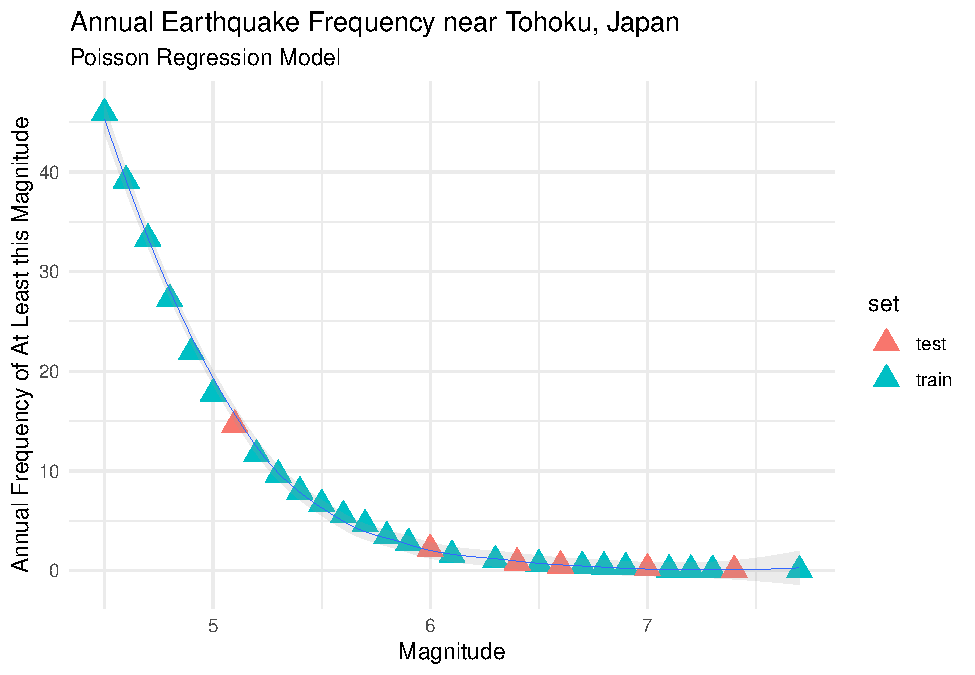
\includegraphics{Appendix_eq_files/figure-latex/unnamed-chunk-3-1.pdf}

\begin{Shaded}
\begin{Highlighting}[]
\CommentTok{\# }\AlertTok{TEST}\CommentTok{ ERROR {-} MSE}
\NormalTok{poissontable }\OtherTok{\textless{}{-}} \FunctionTok{data.frame}\NormalTok{(}\AttributeTok{Model =} \StringTok{"Poisson Regression"}\NormalTok{,}
                          \CommentTok{\# Hidden = NA,}
                           \AttributeTok{TestErr =} \FunctionTok{mean}\NormalTok{((test}\SpecialCharTok{$}\NormalTok{freqc }\SpecialCharTok{{-}}\NormalTok{ test}\SpecialCharTok{$}\NormalTok{fitted)}\SpecialCharTok{\^{}}\DecValTok{2}\NormalTok{))}
                           \CommentTok{\#TrainErr =  sum((pois[["residuals"]])\^{}2))}
\NormalTok{poissontable}
\end{Highlighting}
\end{Shaded}

\begin{verbatim}
##                Model   TestErr
## 1 Poisson Regression 0.1167671
\end{verbatim}

Cross validation scheme to generate Test Error for Poisson regression.
Due to the size of the data, distributions of TestError were skewed. So,
median was taken to measure the final CV score for the network.

\begin{Shaded}
\begin{Highlighting}[]
\NormalTok{k }\OtherTok{\textless{}{-}} \DecValTok{500}
\NormalTok{TestErr }\OtherTok{\textless{}{-}} \ConstantTok{NULL}
\NormalTok{H\_med }\OtherTok{\textless{}{-}} \ConstantTok{NULL}


\ControlFlowTok{for}\NormalTok{(i }\ControlFlowTok{in} \DecValTok{1}\SpecialCharTok{:}\NormalTok{k)\{}
\NormalTok{  df }\OtherTok{\textless{}{-}}\NormalTok{ eq[}\FunctionTok{sample}\NormalTok{(}\FunctionTok{nrow}\NormalTok{(eq)), ]}

  \CommentTok{\# Extract 80\% of data into train set and the remaining 20\% in test set}
\NormalTok{  train\_test\_split }\OtherTok{\textless{}{-}} \FloatTok{0.8} \SpecialCharTok{*} \FunctionTok{nrow}\NormalTok{(df)}
\NormalTok{  train }\OtherTok{\textless{}{-}}\NormalTok{ df[}\DecValTok{1}\SpecialCharTok{:}\NormalTok{train\_test\_split,]}
\NormalTok{  test }\OtherTok{\textless{}{-}}\NormalTok{ df[(train\_test\_split}\SpecialCharTok{+}\DecValTok{1}\NormalTok{)}\SpecialCharTok{:} \FunctionTok{nrow}\NormalTok{(df),]}

\NormalTok{  pois }\OtherTok{\textless{}{-}} \FunctionTok{glm}\NormalTok{(freqc }\SpecialCharTok{\textasciitilde{}}\NormalTok{ mag, }\AttributeTok{data =}\NormalTok{ train, }\AttributeTok{family =} \StringTok{"poisson"}\NormalTok{)}

  \CommentTok{\#{-}{-}{-}make predictions}
\NormalTok{  testpreds }\OtherTok{\textless{}{-}} \FunctionTok{predict}\NormalTok{(pois, }\AttributeTok{type =} \StringTok{"response"}\NormalTok{, }\AttributeTok{newdata =} \FunctionTok{data.frame}\NormalTok{(}\AttributeTok{mag =}\NormalTok{ test}\SpecialCharTok{$}\NormalTok{mag))}

  \CommentTok{\#{-}{-}{-}Mean difference between predictions and actual values for test set}
\NormalTok{  TestErr[i] }\OtherTok{\textless{}{-}} \FunctionTok{mean}\NormalTok{((test}\SpecialCharTok{$}\NormalTok{freqc }\SpecialCharTok{{-}}\NormalTok{ testpreds)}\SpecialCharTok{\^{}}\DecValTok{2}\NormalTok{) }
\NormalTok{\}}

\NormalTok{H\_med }\OtherTok{\textless{}{-}} \FunctionTok{median}\NormalTok{(TestErr)}
\NormalTok{poissontable\_cv }\OtherTok{\textless{}{-}} \FunctionTok{na.omit}\NormalTok{(}\FunctionTok{data.frame}\NormalTok{(}\AttributeTok{Model =} \StringTok{"Poisson Regression"}\NormalTok{, }\AttributeTok{TestErr =}\NormalTok{ H\_med))}
\NormalTok{poissontable\_cv}
\end{Highlighting}
\end{Shaded}

\begin{verbatim}
##                Model   TestErr
## 1 Poisson Regression 0.2004655
\end{verbatim}

\hypertarget{multi-layer-perceptron}{%
\subsection{\#\# Multi-Layer Perceptron}\label{multi-layer-perceptron}}

Cross validation scheme to measure MLP hidden layer size. Due to
computational limitations, only 50 of each network could be built.

It is found that the network converges faster on the log scale, so the
data is transformed first.

\begin{Shaded}
\begin{Highlighting}[]
\NormalTok{k }\OtherTok{\textless{}{-}} \DecValTok{50}
\NormalTok{TestErr }\OtherTok{\textless{}{-}} \ConstantTok{NULL}
\NormalTok{H }\OtherTok{\textless{}{-}} \ConstantTok{NULL}
\NormalTok{H\_med }\OtherTok{\textless{}{-}} \ConstantTok{NULL}

\ControlFlowTok{for}\NormalTok{(j }\ControlFlowTok{in} \FunctionTok{c}\NormalTok{(}\DecValTok{3}\NormalTok{,}\DecValTok{6}\NormalTok{,}\DecValTok{9}\NormalTok{,}\DecValTok{10}\NormalTok{,}\DecValTok{20}\NormalTok{))\{}

  \ControlFlowTok{for}\NormalTok{(i }\ControlFlowTok{in} \DecValTok{1}\SpecialCharTok{:}\NormalTok{k)\{}
\NormalTok{    df }\OtherTok{\textless{}{-}}\NormalTok{ eq[}\FunctionTok{sample}\NormalTok{(}\FunctionTok{nrow}\NormalTok{(eq)), ]}

    \CommentTok{\# Extract 80\% of data into train set and the remaining 20\% in test set}
\NormalTok{    train\_test\_split }\OtherTok{\textless{}{-}} \FloatTok{0.8} \SpecialCharTok{*} \FunctionTok{nrow}\NormalTok{(df)}
\NormalTok{    train }\OtherTok{\textless{}{-}}\NormalTok{ df[}\DecValTok{1}\SpecialCharTok{:}\NormalTok{train\_test\_split,]}
\NormalTok{    test }\OtherTok{\textless{}{-}}\NormalTok{ df[(train\_test\_split}\SpecialCharTok{+}\DecValTok{1}\NormalTok{)}\SpecialCharTok{:} \FunctionTok{nrow}\NormalTok{(df),]}

\NormalTok{    train}\SpecialCharTok{$}\NormalTok{freqc\_log }\OtherTok{\textless{}{-}} \FunctionTok{log10}\NormalTok{(train}\SpecialCharTok{$}\NormalTok{freqc) }\CommentTok{\#log transform for faster convergence}
    \CommentTok{\# test$set \textless{}{-} "test"}
    \CommentTok{\# train$set \textless{}{-} "train"}

\NormalTok{    mlp }\OtherTok{\textless{}{-}} \FunctionTok{neuralnet}\NormalTok{(freqc\_log }\SpecialCharTok{\textasciitilde{}}\NormalTok{ mag,}
                     \AttributeTok{stepmax =} \FloatTok{1e+06}\NormalTok{,}
                     \AttributeTok{data =}\NormalTok{ train,}
                     \AttributeTok{hidden =} \FunctionTok{c}\NormalTok{(j))}

    \CommentTok{\#{-}{-}{-}exponentiate predictions to coerce back to standard scale}
\NormalTok{    testpreds }\OtherTok{\textless{}{-}} \DecValTok{10}\SpecialCharTok{\^{}}\FunctionTok{predict}\NormalTok{(mlp,}\AttributeTok{newdata =} \FunctionTok{data.frame}\NormalTok{(}\AttributeTok{mag =}\NormalTok{ test}\SpecialCharTok{$}\NormalTok{mag))}

    \CommentTok{\#{-}{-}{-}Mean difference between prediction and actual values for test set}
\NormalTok{    TestErr[i] }\OtherTok{\textless{}{-}} \FunctionTok{mean}\NormalTok{((test}\SpecialCharTok{$}\NormalTok{freqc }\SpecialCharTok{{-}}\NormalTok{ testpreds)}\SpecialCharTok{\^{}}\DecValTok{2}\NormalTok{) }
\NormalTok{  \}}

\NormalTok{  H\_med[j] }\OtherTok{\textless{}{-}} \FunctionTok{median}\NormalTok{(TestErr)}
  

\NormalTok{\}}


\NormalTok{mlptable\_cv }\OtherTok{\textless{}{-}} \FunctionTok{na.omit}\NormalTok{(}\FunctionTok{data.frame}\NormalTok{(}\AttributeTok{Model =} \StringTok{"MLP"}\NormalTok{, }\AttributeTok{TestErr =}\NormalTok{ H\_med))}
\NormalTok{mlptable\_cv}
\end{Highlighting}
\end{Shaded}

\begin{verbatim}
##    Model   TestErr
## 3    MLP 0.1845437
## 6    MLP 0.1935333
## 9    MLP 0.2773531
## 10   MLP 0.2902641
## 20   MLP 0.3722027
\end{verbatim}

Code to generate each size MLP

\hypertarget{note-on-mlp-for-count-data}{%
\subsubsection{Note on MLP for count
data}\label{note-on-mlp-for-count-data}}

It is worth noting here that a comparable MLP model to Poisson
regression may be more appropriate for the task at hand. Particularly,
the networks used in \cite{fallah2009nonlinear} to compare the
performance of a neural network Poisson regression model with its
traditional counterpart among various data sets were attempted for this
example. According to the paper, a two-layer neural network is used that
uses hyperbolic tangent in the hidden layer and the exponential function
in the output. To accommodate count data, the loss function based on
negative log likelihood criterion for Poisson regression is: \[
E_D = - \sum_{i=1}^N \left[ -\hat{y_i} + y_i log(\hat{y_i}) \right]
\]

And so the code for the \texttt{neuralnets} package would look as
follows:

\begin{Shaded}
\begin{Highlighting}[]
\NormalTok{mlp }\OtherTok{\textless{}{-}} \FunctionTok{neuralnet}\NormalTok{(freqc }\SpecialCharTok{\textasciitilde{}}\NormalTok{ mag,}
                 \AttributeTok{stepmax =} \FloatTok{1e+06}\NormalTok{,}
                 \AttributeTok{data =}\NormalTok{ train,}
                 \AttributeTok{hidden =} \FunctionTok{c}\NormalTok{(}\DecValTok{5}\NormalTok{),}
                 \AttributeTok{act.fct =} \StringTok{"tanh"}\NormalTok{,}
                 \AttributeTok{err.fct =} \ControlFlowTok{function}\NormalTok{(x, y) \{ }\SpecialCharTok{{-}}\NormalTok{(}\SpecialCharTok{{-}}\NormalTok{x}\SpecialCharTok{+}\NormalTok{y}\SpecialCharTok{*}\FunctionTok{log}\NormalTok{(x))\})}

\NormalTok{predictions }\OtherTok{\textless{}{-}} \FunctionTok{predict}\NormalTok{(mlp, }\AttributeTok{newdata =} \FunctionTok{data.frame}\NormalTok{(}\AttributeTok{mag =}\NormalTok{ test}\SpecialCharTok{$}\NormalTok{mag)) }\SpecialCharTok{\%\textgreater{}\%} \FunctionTok{exp}\NormalTok{()}
\end{Highlighting}
\end{Shaded}

\hypertarget{bayesian-reguarized-neural-network}{%
\subsection{Bayesian Reguarized Neural
Network}\label{bayesian-reguarized-neural-network}}

Using the \texttt{brnn} package \cite{brnn} to create the ideal
two-layer neural network with several simulated trials. Due to
computational limitations, only 50 of each network could be built.

\begin{Shaded}
\begin{Highlighting}[]
\NormalTok{k }\OtherTok{\textless{}{-}} \DecValTok{50}
\NormalTok{TestErr }\OtherTok{\textless{}{-}} \ConstantTok{NULL}
\NormalTok{H\_med }\OtherTok{\textless{}{-}} \ConstantTok{NULL}

\ControlFlowTok{for}\NormalTok{(j }\ControlFlowTok{in} \FunctionTok{c}\NormalTok{(}\DecValTok{3}\NormalTok{,}\DecValTok{6}\NormalTok{,}\DecValTok{9}\NormalTok{,}\DecValTok{10}\NormalTok{,}\DecValTok{20}\NormalTok{,}\DecValTok{50}\NormalTok{))\{}

  \ControlFlowTok{for}\NormalTok{(i }\ControlFlowTok{in} \DecValTok{1}\SpecialCharTok{:}\NormalTok{k)\{}
\NormalTok{    df }\OtherTok{\textless{}{-}}\NormalTok{ eq[}\FunctionTok{sample}\NormalTok{(}\FunctionTok{nrow}\NormalTok{(eq)), ]}

    \CommentTok{\# Extract 80\% of data into train set and the remaining 20\% in test set}
\NormalTok{    train\_test\_split }\OtherTok{\textless{}{-}} \FloatTok{0.8} \SpecialCharTok{*} \FunctionTok{nrow}\NormalTok{(df)}
\NormalTok{    train }\OtherTok{\textless{}{-}}\NormalTok{ df[}\DecValTok{1}\SpecialCharTok{:}\NormalTok{train\_test\_split,]}
\NormalTok{    test }\OtherTok{\textless{}{-}}\NormalTok{ df[(train\_test\_split}\SpecialCharTok{+}\DecValTok{1}\NormalTok{)}\SpecialCharTok{:} \FunctionTok{nrow}\NormalTok{(df),]}
    
\NormalTok{    x }\OtherTok{\textless{}{-}}\NormalTok{ train}\SpecialCharTok{$}\NormalTok{mag}
\NormalTok{    y }\OtherTok{\textless{}{-}}\NormalTok{ train}\SpecialCharTok{$}\NormalTok{freqc }\SpecialCharTok{\%\textgreater{}\%} \FunctionTok{log10}\NormalTok{()}

    \CommentTok{\#{-}{-}{-}build the model with hidden layer size i}
\NormalTok{    brnn }\OtherTok{\textless{}{-}} \FunctionTok{brnn}\NormalTok{(y}\SpecialCharTok{\textasciitilde{}}\NormalTok{x,}\AttributeTok{neurons=}\NormalTok{j)}

    \CommentTok{\#{-}{-}{-}predictions}
\NormalTok{    testpreds }\OtherTok{\textless{}{-}} \DecValTok{10}\SpecialCharTok{\^{}}\FunctionTok{predict}\NormalTok{(brnn, }\AttributeTok{newdata =} \FunctionTok{data.frame}\NormalTok{(}\AttributeTok{x =}\NormalTok{ test}\SpecialCharTok{$}\NormalTok{mag))}

    \CommentTok{\#{-}{-}{-}Mean difference between prediction and actual values for test set}
\NormalTok{    TestErr[i] }\OtherTok{\textless{}{-}} \FunctionTok{mean}\NormalTok{((test}\SpecialCharTok{$}\NormalTok{freqc }\SpecialCharTok{{-}}\NormalTok{ testpreds)}\SpecialCharTok{\^{}}\DecValTok{2}\NormalTok{) }
\NormalTok{  \}}

\NormalTok{H\_med[j] }\OtherTok{\textless{}{-}} \FunctionTok{median}\NormalTok{(TestErr)}

\NormalTok{\}}
\end{Highlighting}
\end{Shaded}

\begin{Shaded}
\begin{Highlighting}[]
\NormalTok{brnntable\_cv }\OtherTok{\textless{}{-}} \FunctionTok{na.omit}\NormalTok{(}\FunctionTok{data.frame}\NormalTok{(}\AttributeTok{Model =} \StringTok{"BRNN"}\NormalTok{, }\AttributeTok{TestErr =}\NormalTok{ H\_med))}
\NormalTok{brnntable\_cv}
\end{Highlighting}
\end{Shaded}

\begin{verbatim}
##    Model    TestErr
## 3   BRNN 0.18900875
## 6   BRNN 0.13294497
## 9   BRNN 0.15097140
## 10  BRNN 0.20731268
## 20  BRNN 0.04056624
## 50  BRNN 0.45928658
\end{verbatim}

Out of all network sizes tested, the best has 20 neurons in the hidden
layer.

\hypertarget{plot-for-brnn}{%
\subsubsection{Plot for BRNN}\label{plot-for-brnn}}

\begin{Shaded}
\begin{Highlighting}[]
\NormalTok{brnn }\OtherTok{\textless{}{-}} \FunctionTok{brnn}\NormalTok{(y}\SpecialCharTok{\textasciitilde{}}\NormalTok{x,}\AttributeTok{neurons=}\DecValTok{20}\NormalTok{)   }\CommentTok{\# build model}
\end{Highlighting}
\end{Shaded}

\begin{verbatim}
## Number of parameters (weights and biases) to estimate: 60 
## Nguyen-Widrow method
## Scaling factor= 14 
## gamma= 9.5446     alpha= 0.0432   beta= 727.4973
\end{verbatim}

\begin{Shaded}
\begin{Highlighting}[]
\FunctionTok{summary}\NormalTok{(brnn)                  }\CommentTok{\# summary of model}
\end{Highlighting}
\end{Shaded}

\begin{verbatim}
## A Bayesian regularized neural network 
## 1 - 20 - 1 with 60 weights, biases and connection strengths
## Inputs and output were  normalized
## Training finished because  SCE <= 0.01
\end{verbatim}

\begin{Shaded}
\begin{Highlighting}[]
\NormalTok{test}\SpecialCharTok{$}\NormalTok{set }\OtherTok{\textless{}{-}} \StringTok{"test"}
\NormalTok{train}\SpecialCharTok{$}\NormalTok{set }\OtherTok{\textless{}{-}} \StringTok{"train"}

\CommentTok{\#{-}{-}{-}append relevant predictions to the training and test datasets}
\NormalTok{test}\SpecialCharTok{$}\NormalTok{brnnpreds }\OtherTok{\textless{}{-}} \DecValTok{10}\SpecialCharTok{\^{}}\FunctionTok{predict}\NormalTok{(brnn, }\AttributeTok{newdata =} \FunctionTok{data.frame}\NormalTok{(}\AttributeTok{x =}\NormalTok{ test}\SpecialCharTok{$}\NormalTok{mag))}
\NormalTok{train}\SpecialCharTok{$}\NormalTok{brnnpreds }\OtherTok{\textless{}{-}} \DecValTok{10}\SpecialCharTok{\^{}}\FunctionTok{predict}\NormalTok{(brnn, }\AttributeTok{newdata =} \FunctionTok{data.frame}\NormalTok{(}\AttributeTok{x =}\NormalTok{ train}\SpecialCharTok{$}\NormalTok{mag))}

\CommentTok{\#{-}{-}combine data sets for plot}
\NormalTok{plot\_brnn }\OtherTok{\textless{}{-}}\NormalTok{ train[,}\FunctionTok{c}\NormalTok{(}\StringTok{"mag"}\NormalTok{,}\StringTok{"freqc"}\NormalTok{,}\StringTok{"set"}\NormalTok{,}\StringTok{"brnnpreds"}\NormalTok{)] }\SpecialCharTok{\%\textgreater{}\%}
            \FunctionTok{rbind}\NormalTok{(test[,}\FunctionTok{c}\NormalTok{(}\StringTok{"mag"}\NormalTok{,}\StringTok{"freqc"}\NormalTok{,}\StringTok{"set"}\NormalTok{,}\StringTok{"brnnpreds"}\NormalTok{)])}

\CommentTok{\#{-}{-}{-}plot the data}
\FunctionTok{ggplot}\NormalTok{(plot\_brnn, }\FunctionTok{aes}\NormalTok{(}\AttributeTok{x =}\NormalTok{ mag)) }\SpecialCharTok{+}
  \FunctionTok{geom\_point}\NormalTok{(}\AttributeTok{size =} \DecValTok{4}\NormalTok{, }\AttributeTok{shape =} \DecValTok{17}\NormalTok{, }\FunctionTok{aes}\NormalTok{(}\AttributeTok{y =}\NormalTok{ freqc, }\AttributeTok{color =}\NormalTok{ set)) }\SpecialCharTok{+}
  \FunctionTok{geom\_smooth}\NormalTok{(}\FunctionTok{aes}\NormalTok{(}\AttributeTok{y =}\NormalTok{ brnnpreds), }\AttributeTok{size =}\NormalTok{ .}\DecValTok{2}\NormalTok{, }\AttributeTok{alpha =}\NormalTok{ .}\DecValTok{2}\NormalTok{) }\SpecialCharTok{+}
  \FunctionTok{theme\_minimal}\NormalTok{() }\SpecialCharTok{+}
  \FunctionTok{labs}\NormalTok{(}\AttributeTok{x =} \StringTok{"Magnitude"}\NormalTok{,}
       \AttributeTok{y =} \StringTok{"Annual Frequency of At Least this Magnitude"}\NormalTok{,}
       \AttributeTok{title =} \StringTok{"Annual Earthquake Frequency near Tohoku, Japan"}\NormalTok{,}
       \AttributeTok{subtitle =} \StringTok{"Two{-}Layer Multi{-}Layer Perceptron with Bayesian Regularization"}\NormalTok{)}
\end{Highlighting}
\end{Shaded}

\begin{verbatim}
## `geom_smooth()` using method = 'loess' and formula = 'y ~ x'
\end{verbatim}

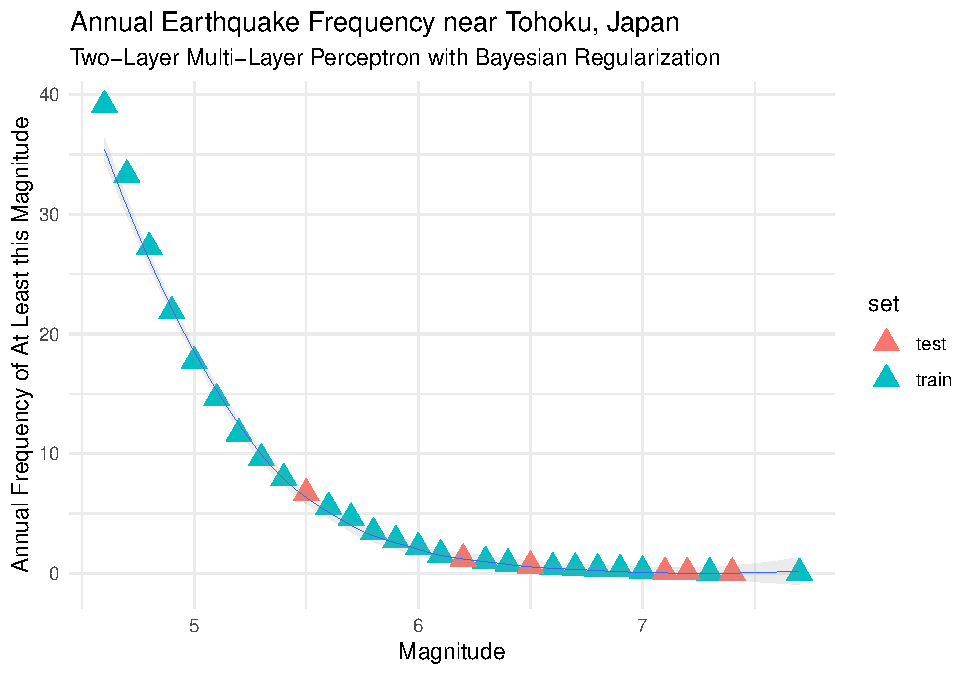
\includegraphics{Appendix_eq_files/figure-latex/unnamed-chunk-14-1.pdf}

\begin{Shaded}
\begin{Highlighting}[]
\FunctionTok{rbind}\NormalTok{(poissontable\_cv,mlptable\_cv,brnntable\_cv)}
\end{Highlighting}
\end{Shaded}

\begin{verbatim}
##                  Model    TestErr
## 1   Poisson Regression 0.20046549
## 3                  MLP 0.18454369
## 6                  MLP 0.19353330
## 9                  MLP 0.27735309
## 10                 MLP 0.29026406
## 20                 MLP 0.37220274
## 31                BRNN 0.18900875
## 61                BRNN 0.13294497
## 91                BRNN 0.15097140
## 101               BRNN 0.20731268
## 201               BRNN 0.04056624
## 50                BRNN 0.45928658
\end{verbatim}

\begin{Shaded}
\begin{Highlighting}[]
\CommentTok{\#\%\textgreater{}\% xtable()}
\end{Highlighting}
\end{Shaded}

I guess this is my punch line now\ldots{}

Simulating 1000 networks' predictions for relative magnitudes with
\emph{neurons = 20}.

\begin{Shaded}
\begin{Highlighting}[]
\CommentTok{\# initialize values}
\NormalTok{x }\OtherTok{\textless{}{-}}\NormalTok{ train}\SpecialCharTok{$}\NormalTok{mag}
\NormalTok{y }\OtherTok{\textless{}{-}}\NormalTok{ train}\SpecialCharTok{$}\NormalTok{freqc }\SpecialCharTok{\%\textgreater{}\%} \FunctionTok{log10}\NormalTok{()}
\NormalTok{n }\OtherTok{\textless{}{-}} \DecValTok{1000}
\NormalTok{prediction\_6}\FloatTok{.1} \OtherTok{\textless{}{-}} \ConstantTok{NULL}

\CommentTok{\# run model and generate predcition n times}
\ControlFlowTok{for}\NormalTok{(i }\ControlFlowTok{in} \DecValTok{1}\SpecialCharTok{:}\NormalTok{n)\{}

\NormalTok{  brnn }\OtherTok{\textless{}{-}} \FunctionTok{brnn}\NormalTok{(y}\SpecialCharTok{\textasciitilde{}}\NormalTok{x,}\AttributeTok{neurons=}\DecValTok{20}\NormalTok{)}

  \CommentTok{\#{-}{-}{-}exponentiate predictions to coerce back to standard scale}
\CommentTok{\#  prediction\_9.1[i] \textless{}{-} 10\^{}predict(brnn, newdata = data.frame(x = 9.1))}
\NormalTok{  prediction\_6}\FloatTok{.1}\NormalTok{[i] }\OtherTok{\textless{}{-}} \DecValTok{10}\SpecialCharTok{\^{}}\FunctionTok{predict}\NormalTok{(brnn, }\AttributeTok{newdata =} \FunctionTok{data.frame}\NormalTok{(}\AttributeTok{x =} \FloatTok{6.1}\NormalTok{))}
\NormalTok{\}}

\NormalTok{ddf\_6}\FloatTok{.1} \OtherTok{\textless{}{-}} \FunctionTok{data.frame}\NormalTok{(}\AttributeTok{iteration =} \DecValTok{1}\SpecialCharTok{:}\DecValTok{1000}\NormalTok{, prediction\_6}\FloatTok{.1}\NormalTok{)}
\end{Highlighting}
\end{Shaded}

\begin{Shaded}
\begin{Highlighting}[]
\CommentTok{\#{-}{-}{-}posterior predictive distribution of a magnitude 6.1}
\FunctionTok{ggplot}\NormalTok{(ddf\_6}\FloatTok{.1}\NormalTok{, }\FunctionTok{aes}\NormalTok{(}\AttributeTok{x =}\NormalTok{ prediction\_6}\FloatTok{.1}\NormalTok{)) }\SpecialCharTok{+}
\FunctionTok{geom\_density}\NormalTok{() }\SpecialCharTok{+}
    \FunctionTok{labs}\NormalTok{(}\AttributeTok{x =} \StringTok{"Predicted Annual Frequency"}\NormalTok{,}
         \AttributeTok{y =} \StringTok{"Density"}\NormalTok{,}
         \AttributeTok{title =} \StringTok{"Approximate Posterior Predictive Density of a Magnitude 6.1 Earthquake"}\NormalTok{,}
         \AttributeTok{subtitle =} \StringTok{"Two{-}Layer Neural Network with Bayesian Regularization"}\NormalTok{) }\SpecialCharTok{+}
  \FunctionTok{theme\_minimal}\NormalTok{()}
\end{Highlighting}
\end{Shaded}

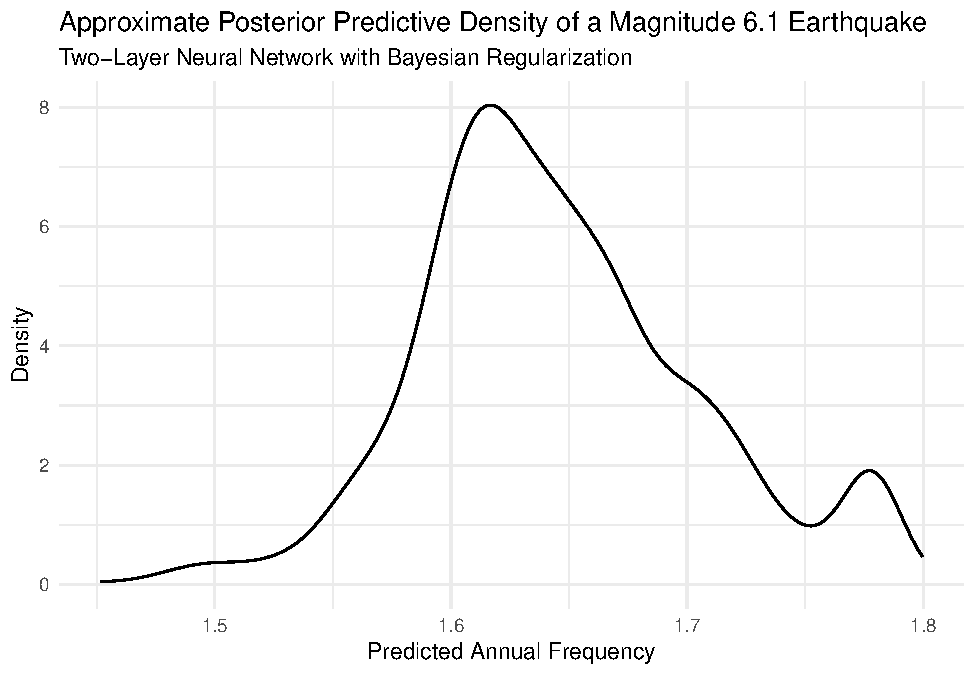
\includegraphics{Appendix_eq_files/figure-latex/unnamed-chunk-17-1.pdf}

\end{document}
